\section{The Human Visual System and Attention}
\label{sec:HVS_attention}

\subsection{The Human Visual System}

A simplified model puts the field of view to around 200° to 220° horizontally and around 125° vertically with the vertical field extending slightly more downwards [\cite{loschkyScenePerceptionCentral2017}]. The central vision covers about 5° around the point of fixation, where acuity is highest [\cite{loschkyScenePerceptionCentral2017}, \cite{rosenholtzCapabilitiesLimitationsPeripheral2016}]. The remaining field is the periphery, with boundaries at 30° and 60° dividing it into near, mid and far peripheral vision.

\begin{figure}[hbt]
    \centering
    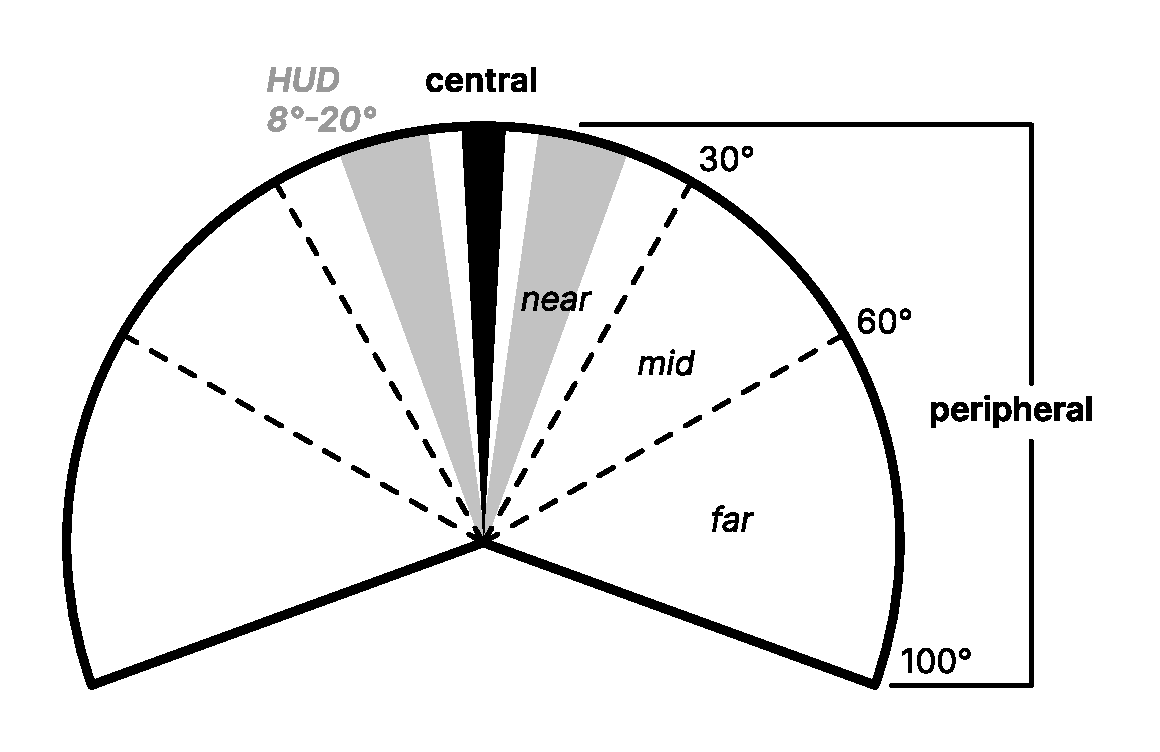
\includegraphics[width=0.5\textwidth]{assets/FOV.eps}
    \caption{Simplified diagram of the field of view.}
    \label{fig:FOV}
\end{figure}

Despite changing anatomical structure from center of gaze to periphery, entire scene appears in high resolution, contrast, color saturation \cite{loschkyScenePerceptionCentral2017}. 

Perception does not require a lot of details, the recognition of abjects and orienting oneself ist still possible [\cite{rosenholtzCapabilitiesLimitationsPeripheral2016}]. That is why image thumbnails are still recognizable.

\textcite{rosenholtzCapabilitiesLimitationsPeripheral2016} suggests that crowding is the biggest issue when it comes to parsing information. The effect is more intense if the target and its neighboring elements are similar (e.g. the same color and shape) [\cite{pelliUncrowdedWindowObject2008}]. The farther away elements are from the center of vision, the bigger the distance between elements has to be.

% GRAPHIC include fig 4 of ROSENHOLTZ 1016? The letters placed close together are perceived as one unit rather than three.
% \cite{pelliUncrowdedWindowObject2008} has a lot of examples

The peripheral vision is good at detecting motion, provides better sight in low light conditions [\cite{johnsonChapter5Our2014}] and contributes to functions like orientation, navigation, balance and hand-eye coordination. Restricting the peripheral vision affects all of these negatively, getting worse the more is occluded, severely impacting performance \cite{alfanoRestrictingFieldView1990}.

Color sensitivity decreases toward the periphery, red-green moreso than blue-yellow colors and sensitivity to luminance. \textcite{hansenColorPerceptionIntermediate2009} found that as long as the stimulus is of sufficient size, perceiving color is possible even at 50° eccentricity. Most modern OST-HMDs feature a 40° field of view, meaning the full available color spectrum can be used.

\subsection{Visual Attention}

The perception of images generates too big an amount of information to process at once. This bottle neck is solved by visual attention: limiting the processing by focusing on just a fragment of the current visual stimuli [\cite{andersonDirectedVisualAttention2005}, \cite{rosenholtzCapabilitiesLimitationsPeripheral2016}]. This process is guided by the peripheral vision, subconsciously preselecting salient features of the environment [\cite{}]. Saliency describes features which make a target differ from surrounding objects [\cite{johnsonChapter5Our2014}].
% -> visual hierarchy
% -> non-linear visual search

\cite{rosenholtzCapabilitiesLimitationsPeripheral2016}
- “Because of the brain's limited capacity, our visual systems cannot automatically perform every possible visual task at the same time. Instead, the brain may concentrate resources on one task in a given moment, then switch to focus on another task.”
- “Our results suggest that the visual system looks for evidence of a change throughout the visual field, possibly in parallel, rather than looking for a change merely where one fixates. However, that evidence of a change can be weak because of loss of information in peripheral vision, making change detection difficult.”

\cite{caterSelectiveQualityRendering2002}
- process by which we humans select a portion of the available visual information for localization, identification, and understanding of objects in an environment
- allows the visual system to process visual input preferentially by shifting attention about an image, giving more attention to salient locations and less attention to unimportant regions

% GRAPHIC perception pipeline: perception, attention as filter, cognition

% Saccades: fast, scanning movements, Fixations: eye focuses on one spot to comprehend, metrics for attention: fixation duration, frequency

% habituation: less attention to any stimulus that occurs frequently

There are two ways in which an object can be focused: bottom-up and top-down. Bottom-up attention is subconscious, stimulus driven. For the top-down process, the brain directs the eyes to focus on a consciously chosen object. Interestingly, when concentrating on an objective, the top-down attention lessens the effect of distracting stimuli [\cite{connorVisualAttentionBottomUp2004}].

If multiple stimuli compete for attention, even salient targets might be ignored, if they are irrelevant to the current objective. This is called inattentional blindness [\cite{jensenChangeBlindnessInattentional2011}]. This effect can be leveraged, for example \textcite{caterSelectiveQualityRendering2002} who use it to only render high quality images in the center of vision.
